\documentclass[a4paper, fleqn]{article}
\usepackage{header}

\title{Семинарский лист 2.4}
\author{
    % Александр Богданов   \\ \href{https://t.me/SphericalPotatoInVacuum}{Telegram} \and
    % Алиса Вернигор       \\ \href{https://t.me/allisyonok}{Telegram} \and
    % Анастасия Григорьева \\ \href{https://t.me/weifoll}{Telegram} \and
    % Василий Шныпко       \\ \href{https://t.me/yourvash}{Telegram} \and
    % Данил Казанцев       \\ \href{https://t.me/vserosbuybuy}{Telegram} \and
    % Денис Козлов         \\ \href{https://t.me/DKozl50}{Telegram} \and
    % Елизавета Орешонок   \\ \href{https://t.me/eaoresh}{Telegram} \and
    % Иван Пешехонов       \\ \href{https://t.me/JohanDDC}{Telegram} \and
    % Иван Добросовестнов  \\ \href{https://t.me/ivankot13}{Telegram} \and
    % Настя Городилова     \\ \href{https://t.me/nastygorodi}{Telegram} \and
    % Никита Насонков      \\ \href{https://t.me/nnv_nick}{Telegram} \and
    % Сергей Лоптев        \\ \href{https://t.me/beast_sl}{Telegram}
}

\date{Версия от {\ddmmyyyydate\today} \currenttime}

\begin{document}
    \maketitle
   
    \section*{Предполагая функцию $f$ непрерывной на $D$, запишите тройной интеграл от $f$ по $D$ в виде
    одного из повторных, если $D$ задано неравенствами.}
    
    \subsection*{Задача 1} 
    
    $0 \leq z \leq 4 - x^2, \; x^2 - y^2 \geq 0, \; x \geq 0. $
    
    Хочу интегрировать в порядке $\displaystyle \int \limits_{\dots}^{\dots} dx \int \limits_{\dots}^{\dots} dy \int \limits_{\dots}^{\dots} f(x, y, x) dz.$
    
    Посмотрим, что происходит при фиксированном $x$.
    
    Так как $x^2 \geq y^2 \iff |x| \geq |y|,$ то $-x \leq y \leq x \;  $ ($x$ положительный). Ещё знаем, что $0 \leq z \leq 4 -x^2.$
    
    Итак,  $\displaystyle \int \limits_{\dots}^{\dots} dx \int \limits_{-x}^{x} dy \int \limits_{0}^{4 -x^2} f(x, y, x) dz.$ 
    
    А каковы границы $x$? $x \geq 0$, это нам дано. Из того, что $z \in [0, 4 -x^2]$, сделаем вывод, что $x \leq 2$, ведь при больших значениях $x$ множество становится вырожденным.
    
    Так что границы интегрирования знаем,  $\boxed{\displaystyle \int \limits_{0}^{2} dx \int \limits_{-x}^{x} dy \int \limits_{0}^{4 -x^2} f(x, y, x) dz} \; .$ 
    
    
    % \subsection*{Задача 2}
    
    \subsection*{Задача 3}
    
    $0 \leq z \leq 4xy, \; x + 4y + z \leq 1. $
    
    
    
    % \subsection*{Задача 4}
    
    \subsection*{Задача 5}
    
    $x^2 + y^2 \geq 3 z^2, \; x^2 + y^2 - z^2 \leq 2. $
    
    Проинтегрируем внешне по $z$. 
    
    $z = const \implies x^2 + y^2 \geq 3z^2, \; x^2 + y^2 \leq z^2 + 2.$
    
    Нам интересно примерно такое колечко:
    
    
   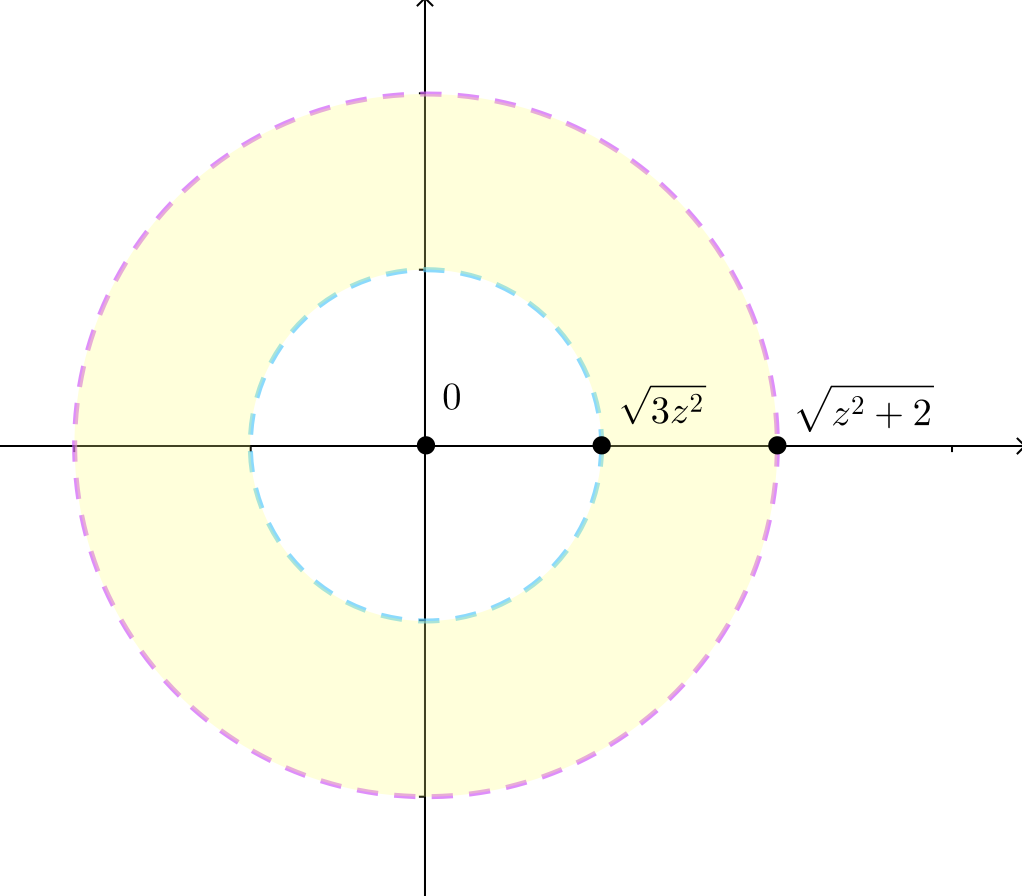
\includegraphics[width=8.5cm, height=8cm]{task 2.4.3.png}
    
    Можно начать разбивать область интегрирования по $x$. Но мы ленивые. Поэтому просто вычтем из площади большей окружности площадь меньшей.
    
    Тогда внутри интеграла по $z$ появится $\displaystyle \int \limits_{-\sqrt{z^2 + 2}}^{\sqrt{z^2 + 2}} dx \int \limits_{-\sqrt{z^2 + 2 - x^2}}^{\sqrt{z^2 + 2 - x^2}} f dy - \int \limits_{-\sqrt{3z^2}}^{\sqrt{3z^2}} dx \int \limits_{-\sqrt{3z^2- x^2}}^{\sqrt{3z^2 - x^2}} f dy  .$
    
    
    Для не-вырожденности множества, получаем условие $\sqrt{3z^2} \leq \sqrt{z^2 + 2} \iff 2z^2 \leq 2 \iff |z| \leq 1 \iff z \in [-1, 1].$
    
    
    Итого $\displaystyle \int \limits_{-1}^{1} dz \left( \; \int \limits_{-\sqrt{z^2 + 2}}^{\sqrt{z^2 + 2}} dx \int \limits_{-\sqrt{z^2 + 2 - x^2}}^{\sqrt{z^2 + 2 - x^2}} f dy - \int \limits_{-\sqrt{3z^2}}^{\sqrt{3z^2}} dx \int \limits_{-\sqrt{3z^2- x^2}}^{\sqrt{3z^2 - x^2}} f dy  \right).$
    
    % \subsection*{Задача 6}
    
    \section*{Вычислите интеграл.}
    \subsection*{Задача 7} 
    
    % \subsection*{Задача 8}
    
    \subsection*{Задача 9}
    
    % \subsection*{Задача 10}
    d
    \section*{Измените порядок интегрирования и вычислите интеграл.}
    
    \subsection*{Задача 11}
    
    % \subsection*{Задача 12}
    
    % \subsection*{Задача 13}
    
    % \subsection*{Задача 14}
    
    % \subsection*{Задача 15}
    
    % \subsection*{Задача 16}
    
    % \subsection*{Задача 17}
    
    \section*{Вычислите многократный интеграл.}
    % \subsection*{Задача 18}
    
    % \subsection*{Задача 19}
    
    % \subsection*{Задача 20}
    
    % \subsection*{Задача 21}
    
    % \subsection*{Задача 22}
    
    % \subsection*{Задача 23}
    
\end{document}
